\chapter{Jätkusuutlik areng}
\section{Konteksti kaardistamine}
Jätkusuutmatus on tihti ühel või teisel viisil seotud ressursi lõppemisega. Miski, millest me sõltume, saab otsa. Järelikult on oluline aru saada, millistest ressurssidest me sõltume ning kes sõltub meist. Seejärel on võimalik uurida, milline on meie jaoks oluliste ressursiallikate taastootmisvõime, kas nad võivad lõppeda ning kuidas me tolles lõppemisest teada võiksime saada\sidenote{Siit järeldub muu hulgas, et meie jaoks liiga keeruliste\index{Keerukus} süsteemide puhul on keeruline rääkida jätkusuutlikkusest. Me lihtsalt ei tea, millest nad sõltuvad ja mil määral}.

Väärtusahel\index{Väärtusahel} on ikka olnud üheks viisiks ärimudelit visualiseerida ja sellest mõelda. Tegu on siiski ka makrotasandil kasuliku vahendiga keeruliste suhtevõrgustike analüüsimiseks. Meetod on lõtv ja vabalt kohaldatav, kuid laias laastus saab talle siiski struktuuri anda. Kontekstikaardistus käib nii. 

Grupp inimesi viib valge tahvliga ruumis läbi järgmised sammud:
\begin{enumerate}
	\item Joonistame üles kõik huvitatud osapooled\sidenote{Sisuliselt kaardistame süsteemi kõik elemendid. Tegemist on \cite{crawley2015systems} kirjeldatud süsteemianalüüsi esimese sammuga: loetleme süsteemi elemendid}. Rahulikult võib ignoreerida osapoolte tüüpe ja omavahelisi hierarhilisi sõltuvusi. Keerukamatel juhtudel võib need eraldi, näiteks teise värviga, välja tuua. Samal pildil võivad eraldi kehad olla töötaja ja tööandja. 
	\item Lähtudes meid kõige enam huvitavast (tavaliselt konkreetse kokkusaamise algataja ning kasusaaja), küsime iga osapoolte paari kohta
		\begin{itemize}
			\item Mida saab osapool A osapoolelt B?
			\item Mida saab osapool B osapoolelt A?
		\end{itemize}
	\item Kõik seosed joonistame üles õiges suunas näitavate nooltega 
	\item Valideerime pildi küsides iga osapoole kohta: "kust na saavad seda, mida nad ära annavad?"
	\item Analüüsime pilti. Näiteks on oluline tuvastada "väravavahid" ehk kahte omavahel tihedalt seotud ökosüsteemi ühendavad graafi tipud
\end{enumerate}

\begin{figure}[h]
	\begin{center}
		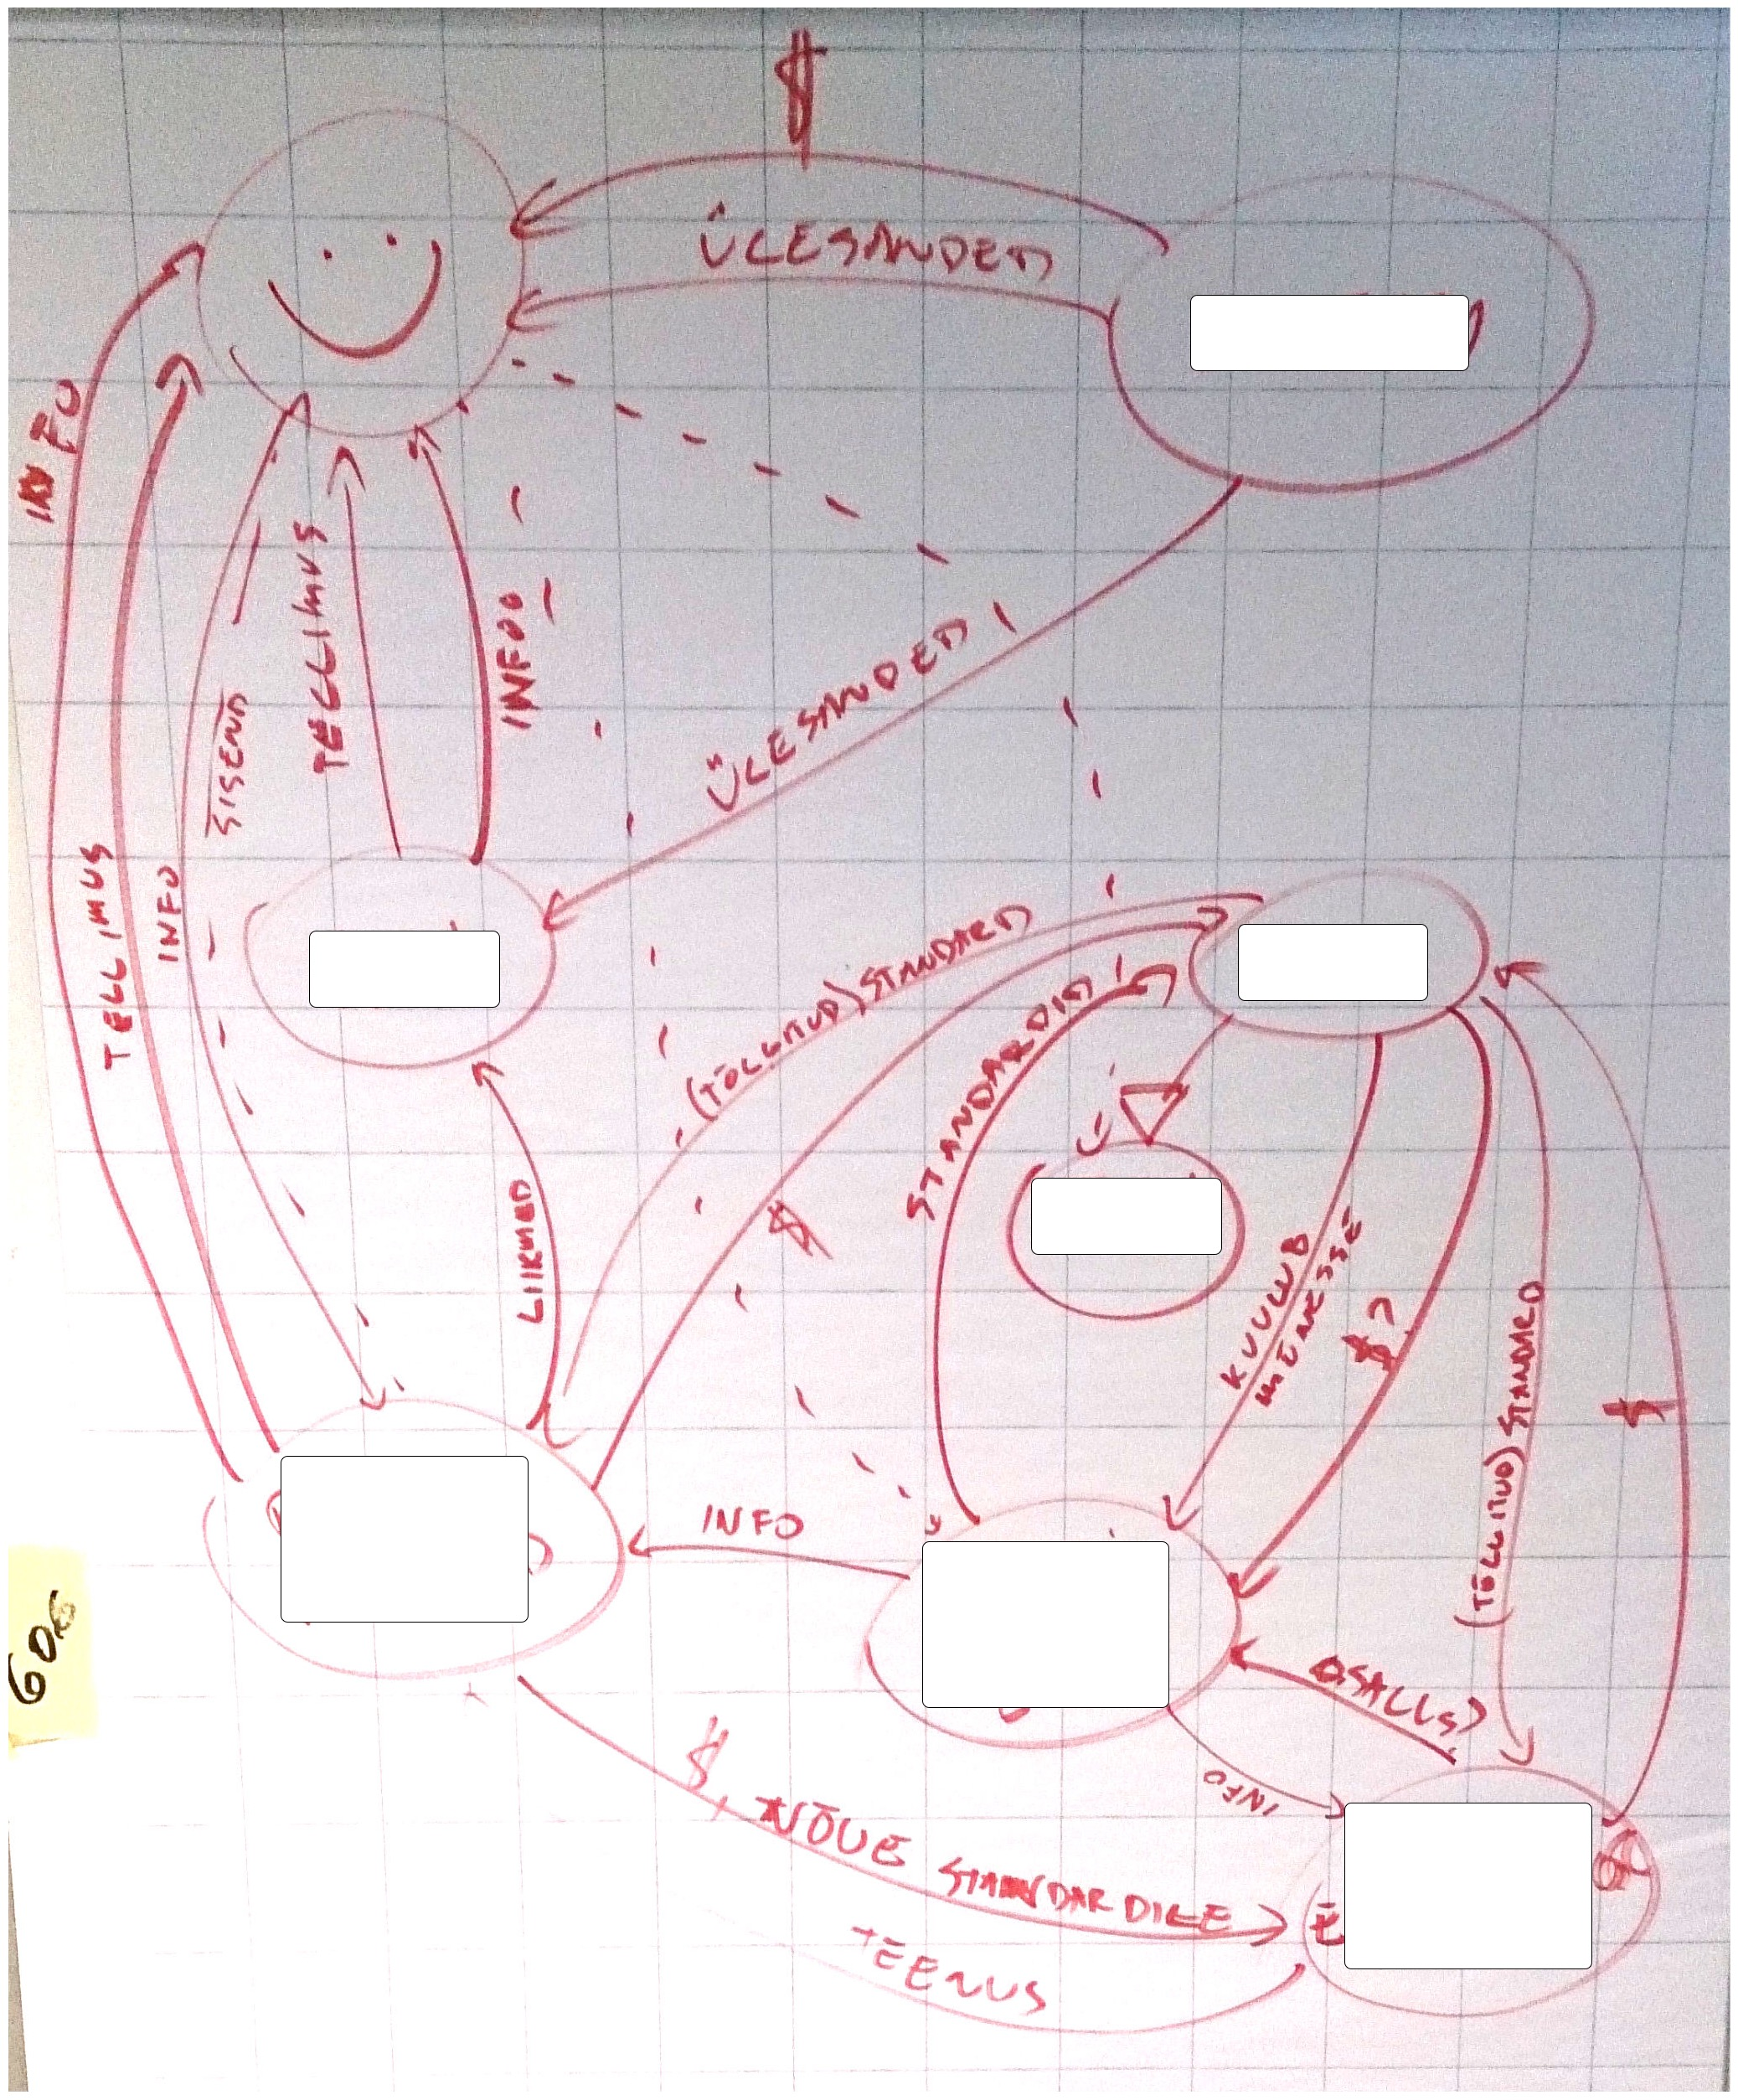
\includegraphics[width=.6\textwidth]{seosed.jpg}
		\caption{Näide seoste diagrammist}
		\label{fig:seosed}
	\end{center}
\end{figure}




\section{Piiridest ja nende ületamisest}
Eelmise sajandi seitsmekümnendatel töötas Jay Forrester Rooma Klubi tellimusel välja mudeli maailma rahvastiku kasvu uurimiseks. Forresteri õpilased on mudelit hiljem täiendanud, hetkel on ehk parim lugemismaterial \cite{meadows1992beyond}. Ennustused ei ole roosilised, pigem vastupidi. Ühe tõenäolise võimalusena nähakse ette, et rahavastik ületab suurelt piirid, mida tehnoloogia võimaldab planeedil Maa ära toita ning mahutada ja et järgneb mõõdukas kollaps. Rahvastik kahaneb kiiresti ning palju ning toimub tugev konkurents ressursside pärast (sest kõigile lihtsalt ei jätku). 

\section{Trammifaktor}
\index{Truck number}
Jätkusuutlikkust võib ka vaadata riskijuhtimise nurga alt. Sel viisil mõeldes on jätkusuutmatu olukord, kus organisatsiooni jaoks kriitiline risk on maandamata. Riskide ignoreerimine võib hästi lõppeda vaid piiratud aja jooksul.

Üheks tüüpiliseks IT-organisatsioonide riskiks on inimrisk. Ikka ja jälle leiame end olukorrast, kus kogu teadmine mingi valdkonna või süsteemi kohta on koondunud ühe inimese pähe\sidenote{Tüüpiliselt on tegemist tagasisidega: Kuna inimene teab süsteemist kõige rohkem, pöördutakse murega tema juurde. Mure lahenemise läbi suureneb tema teadmine süsteemist ja seega ka suhteline kompetents võrreldes teistega. Ja suureneb ka tõenäosus, et ka järgmine kord minnakse probleemiga tema juurde. Ta teab süsteemist seda rohkem, mida rohkem ta süsteemist teab.}. Tegu on niivõrd tüüpilise riskiga, et agiilses arenduses on olemas spetsiaalne termin - \emph{truck number}\cite{coplien2004organizational}. Eesti keelde võiks selle ehk tõlkida kui \enquote{trammifaktori}. Trammifaktor on maksimaalne tiimi liikmete arv, kelle trammi alla jäämine mõjutaks meeskonna jõudlust lineaarselt. Kui trammifaktor on üks, siis mõjutab õnnetus võtmeisiku oluliselt rohkem, kui lihtsalt tema panuse puudumine. Ideaalis on N-liikmelise meeskonna trammifaktor N-1, kuid praktikas nii hästi juhitud meeskondi tihti ei kohta. 

\section{Küsimused aruteluks}
\subsection{Miks on kõrge PUE oluline?}
PUE\sidenote{PUE - \emph{Power usage effectiveness} näitab, milline osa kogu kulutatavast energiast kulutatakse arvutustehnika käitamisele}\index{PUE} on küllalt populaarne viis andmekeskuste efektiivsuse hindamiseks. Kõige ilmselgemalt on tema maksimeerimine kasulik majanduslikult: kui PUE on üks, kulub kogu elektriarve arvutamiseks ja seega väärtuse loomiseks. Samas on PUE kasvatamine ka selgesti kahaneva piirkasulikkusega protsess\sidenote{Iga järgmine ühik PUEd tuleb kallimalt kui eelmine. Tegemist on dünaamiliste süsteemide puhul tavapärase asümptootilise lähenemisega sihile. Ehk, PUE küll saab ideaalile, ühikule, läheneda kuid ei saa ealeski kohale jõuda}. Järelikult nõuab PUE kasvatamine investeeringut. Loogiliselt võttes ei ole mõistlik investeerida rohkem, kui läbi energiasäästu tagasi tuleb\sidenote{Formaalselt tuleb lahendada võrrand $I_0=\sum_{t} \frac{C_t(I_0)}{(1+r)^t}$ $I_0$ jaoks. Ehk, igakuine sääst elektriarvelt peab meid huvitava perioodi jooksul intressimäära r juures võrduma algse investeeringuga. Paraku, nagu öeldud, on $C_t$ mittelineaarne funktsioon ja seega eeldab tasakaalupunkti leidmine tavaliselt suhteliselt keerukat stsenaariumide läbi arvutamist.}. Igasugune nüüdisväärtuse arvutus sõltub olemuslikult ka ajaperioodist ning seega oleme saanud seose ettevõtte toimetamise ajalise perspektiivi ning jätkusuutlikkuse vahel. 

Teine PUE kasvatamise põhjus võib olla keskkonnast tulenev. Kui kogu energia kulutatakse arvutamisele, peaks see ju vähendama organisatsiooni ökoloogilist jalajälge, vähendama koormust keskkonnale? Kindlasti on tegemist olulise põhjusega kuid tuleb teha vahet keskkonnasõbraliku maine ja reaalse keskkonnasõbralikkuse vahel. Nimelt mõõdab PUE energiaefektiivsust vaid andmekeskuse sees. Tuletades meelde diskussiooni süsteemi piiridest\index{Süsteem!Piirid} on lihtne näha probleemi. Nimelt võib küll andmekeskus toimida äärmiselt efektiivselt juhtides arvutamise käigus tekkivad jääksoojust keskkonda, kuid ta ei ütle midagi keskkonnas toimuva kohta. On suhteliselt lihtne disainida soojusvahetusele tuginev süsteem, mis talvel eraldab väga efektiivselt keskkonnas ruumide kütmiseks piisavalt soojust ning suvel viib liigsoojuse sinnasamma tagasi. Kuid kuna arvuti on ikkagi kütteallikas, võib maasse pumbatav energiahulk oluliselt ületada sealt võetava. Põhimõtteliselt köetakse serveriruumi ümbritsevat pinnast ning see ei pruugi ökosüsteemi vaatepunktist kasulik olla. 

Kui nüüd regulaator otsustab näiteks seada PUEle teatud sihtväärtused kuid ei rakenda piiranguid keskkonna mõjutamisele, saame täiesti ebasoovitava tulemuse. Energiatõhususe läbi keskkonnasäästu soovides tekitame keskkonnale koormuse, mille suhe saavutatud kokkuhoidu ei ole sugugi ilmne. Ettevõtte kuvand käitub sarnaselt regulaatoriga. Ka avalikkusel on teatav ootus ettevõtte teatud käitumise suhtes ning oodatud käitumise ning tegeliku kekskonnamõju vahel ei pruugi olla üksühest seost.

Juba suhteliselt lihtsa arutluse käigus ühest serveriruumi efektiivsusnäitaja üle tõusid esile keeruline mittelineaarne optimiseerimisülesanne, dünaamiline keerukus, küsimus ajahorisonidst ja avalikkussuhted. Küsimus terve ettevõtte jätkusuutlikkusest on veelgi keerulisem. 


\subsection{Kuidas tuvastada jätkusuutmatust?}
Lähtudes jätkusuutlikkuse definitsioonist \enquote{jätkusuutlik on tegevus, mida võib mingites ajaraamides sarnaste tulemustega jätkata} on jätkusuutmatuse täielik tuvastamine keeruline. Selleks on definitsioon liiga üldine. Küll aga võib suhteliselt kergesti tuvastada konkreetseid käitumisi, mille jätkusuutmatus tuleneb nende olemusest. Eksponentsiaalne kasv, näiteks, ei saa lõputult jätkuda, varem või hiljem saavad mingid ressursid otsa. Ülesande teeb lihtsamaks asjaolu, et süsteemide probleemid on reeglina endogeensed, seega võime välised tegurid rahulikult kõrvale jätta.

Millised siis on käitumised, mis ei ole olemuslikult jätkusuutlikud? Toetudes Senge\cite{senge19905th} süsteemiarhetüüpidele võib välja joonistada järgmised peamised jätkusuutmatud mustrid
\begin{description}
	\item[Piiratud kasv] Protsess toidab iseennast viies kiireneva kasvu või ekspansioonini. Ühel hetkel hakkab kasv aeglustuma kuni peatub või (ülereageerimise korral) muutub kiirenevaks kahanemiseks. Põhjuseks on üks või mitu välist tasakaalustavat mehhanismi. Näitena võib tuua MySpace'i\sidenote{Asutati 2003. aastal, oli 2005-2008 suurim sotsiaalvõrk maailmas} sotsiaalvõrgustiku. Mida rohkem seal inimesi käis, seda kasulikum oli kontot omada ja seda rohkem inimesi keskkonda ka külastas. Võrgustiku populaarsus aga tekitas järjest kasvava innovatsioonihuvi konkurentide poolt. Kuni ühel hetkel kerkis esile Facebook ning algne kasv pöördus. Mida vähem inimesi MySpace kasutajaks jäi, seda vähem oli seal põhjust käia.
	\item[Eskalatsioon] Kaks osapoolt näevad oma edu suhtelise ülekaaluna teisest. Mida paremaid tulemusi üks osapool saavutab, seda rohkem teine pingutab tõstes oma tulemust mis viib omakorda suurema pingutuseni esimeselt osapoolelt. On selge, et ühel hetkel sekkub piiratud kasvu stsenaarium ning olukord ei ole jätkusuutlik. Siiski on tavaliselt enne lõppu kulutatud palju rohkem ressursse, kui mõistlik oleks. Heaks näiteks eskalatsioonist on külma sõja aegne tuuma-arsenali kuhjamine. Hetkeks, kui Nõukogude süsteemi piirid kätte jõudsid, oli valmis ehitatud oluliselt rohkem relvastust, kui võiks eales sisulist väärtust omada.
	\item[Jagatud ressursi tragöödia] Osapooled kasutavad ühist kuid piiratud ressurssi. Seejuures on ressursikasutus end taastootev. Mida vähemaks jääb ressurssi, seda rohkem pingutatakse selle kasutamiseks ning seda intensiivsemaks ressursikasutus kõigi osapoolte poolt muutub. Lõpuks saab ühine ressurss otsa. Näitena võib tuua IT arenduse. Tavaliselt on tegemist eri osakondade jaoks jagatud ressursiga. Mida rohkem mõni osakond arendust vajab, seda edukam ta on ja seda suurem huvi on majasisese konkurentsi tingimustes ka teistel oma süsteeme arendada. Tulemuseks on IT-arenduse \enquote{pikali jooksmine} ning kõigi osapoolte võimekus midagi tehtud saada.
	
\end{description}

Kindlasti on erisuguseid jätkusuutmatuse näiteid veel, kuid kirjeldatud kolm katavad ära peamised süsteemide tüübid, mis oma käitumist lõputult jätkata ei saa.

